
\documentclass[10pt,xcolor=table]{beamer}
\usepackage[french]{babel}
\usepackage[T1]{fontenc}
\usepackage[utf8]{inputenc}
\usetheme{Warsaw}
\usepackage{pdfpages}

\title{Outil automatique de décryptage}

\begin{document}
\begin{frame}
  \frametitle{Dcrypt}
\begin{center}
\Huge {Outil automatique de décryptage}
\end{center}
\end{frame}


%nico
\begin{frame}
  \frametitle{Introduction}

  \begin{itemize}[<+->]
  \item Definition de Crypto par Ronald Rivest
  
  \begin{block}{Les 3 critères}
    \begin{itemize}
    \item Confidentialité,
    \item Authenticité,
    \item integrité
    \end{itemize}
  \end{block}
  \end{itemize}

\end{frame}


\begin{frame}[<+->]
  \frametitle{Introduction}

  \begin{block}{Phases de développement}
   
    \begin{enumerate}
    \item Identification,
    \item Définition,
    \item Réalisation,
    \item Finalisation
    \end{enumerate}
  \end{block}

\end{frame}
%flo
\begin{frame}
  \frametitle{Organigramme}
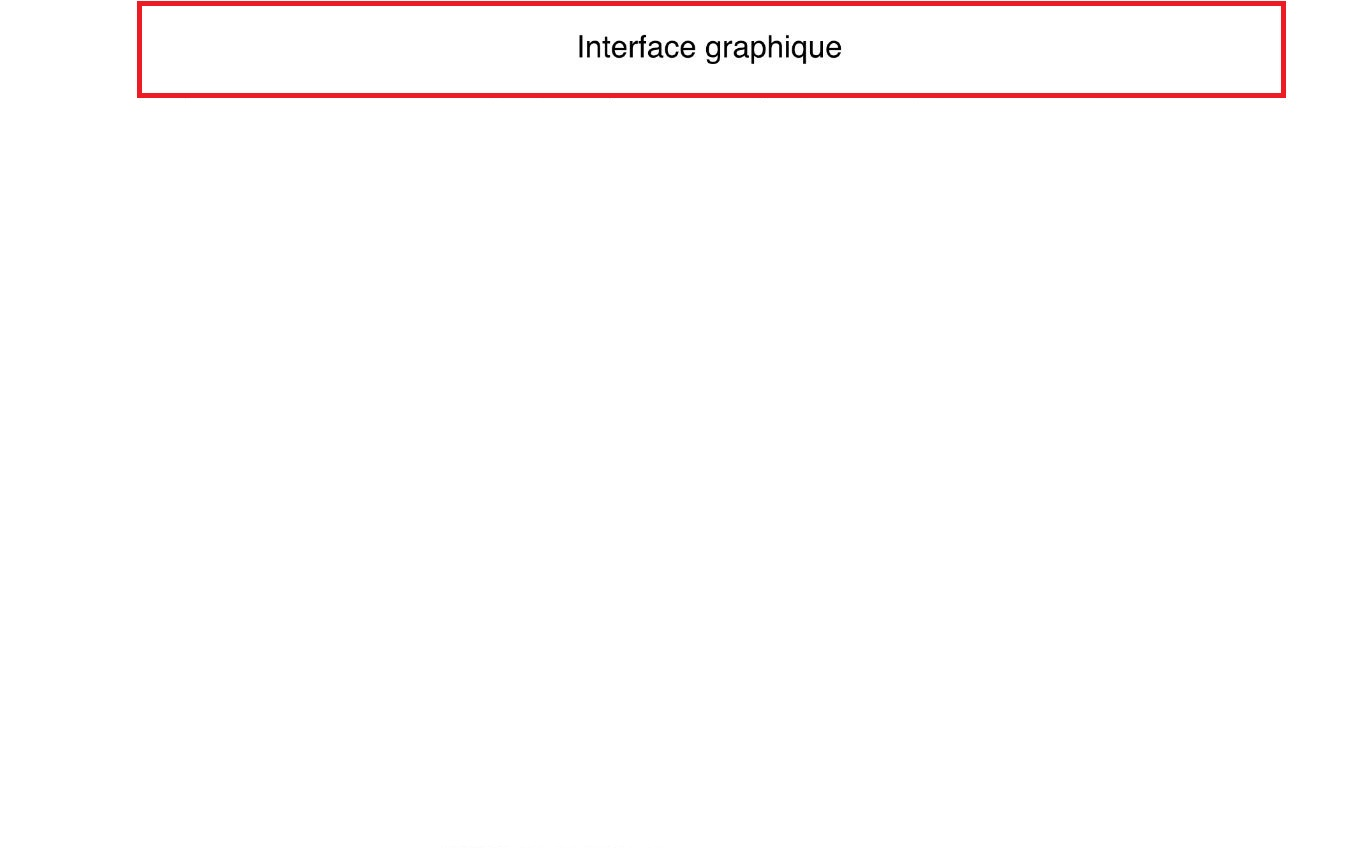
\includegraphics[scale = 0.28]{Org1.jpg}\\
Module principal dont le rôle est de mettre une interface à disposition de l'utilisateur.
\end{frame}
\begin{frame}
  \frametitle{Organigramme}
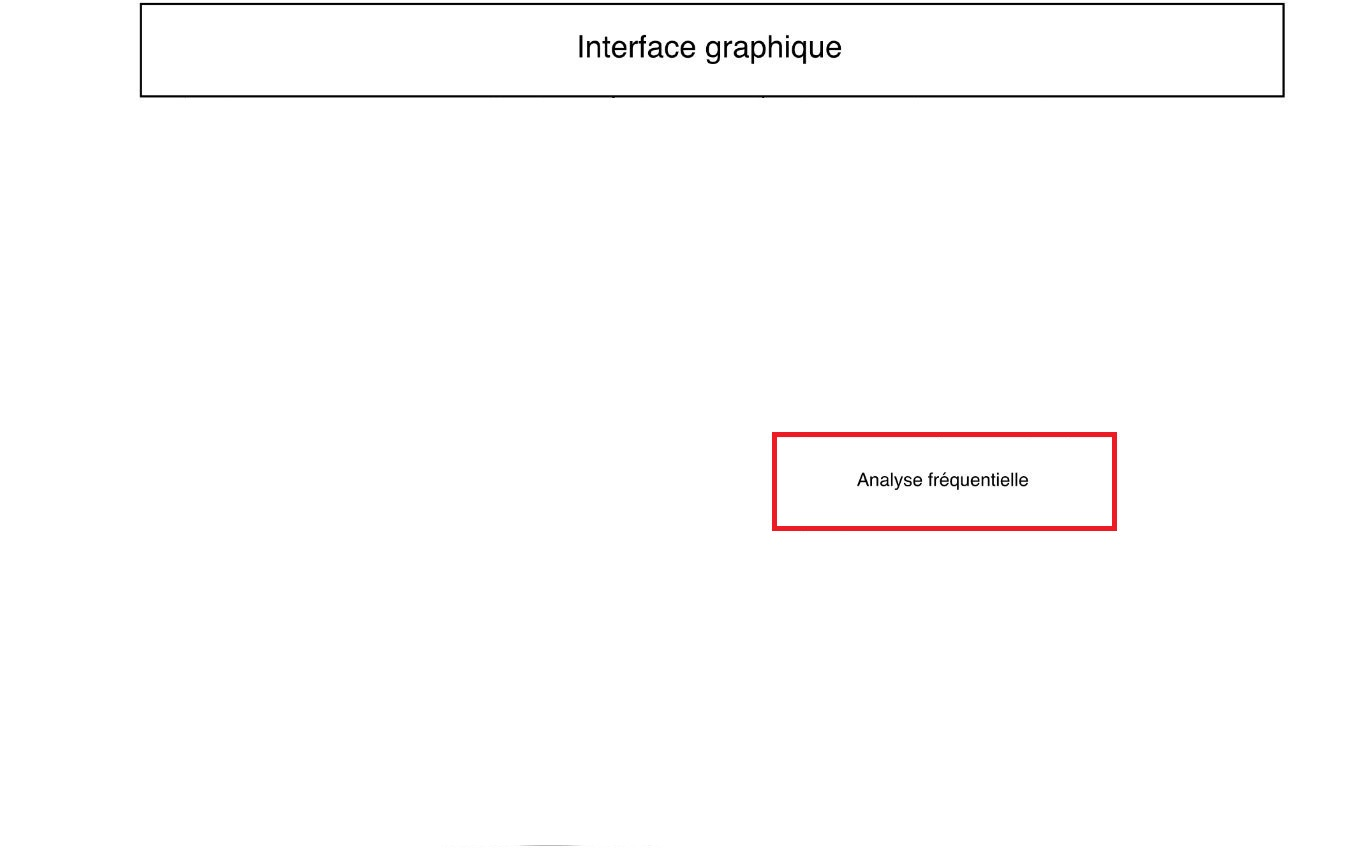
\includegraphics[scale = 0.28]{Org2.jpg}\\
Module qui compte le nombre de caractères, de digrammes et de trigrammes du texte.
\end{frame}
\begin{frame}
  \frametitle{Organigramme}
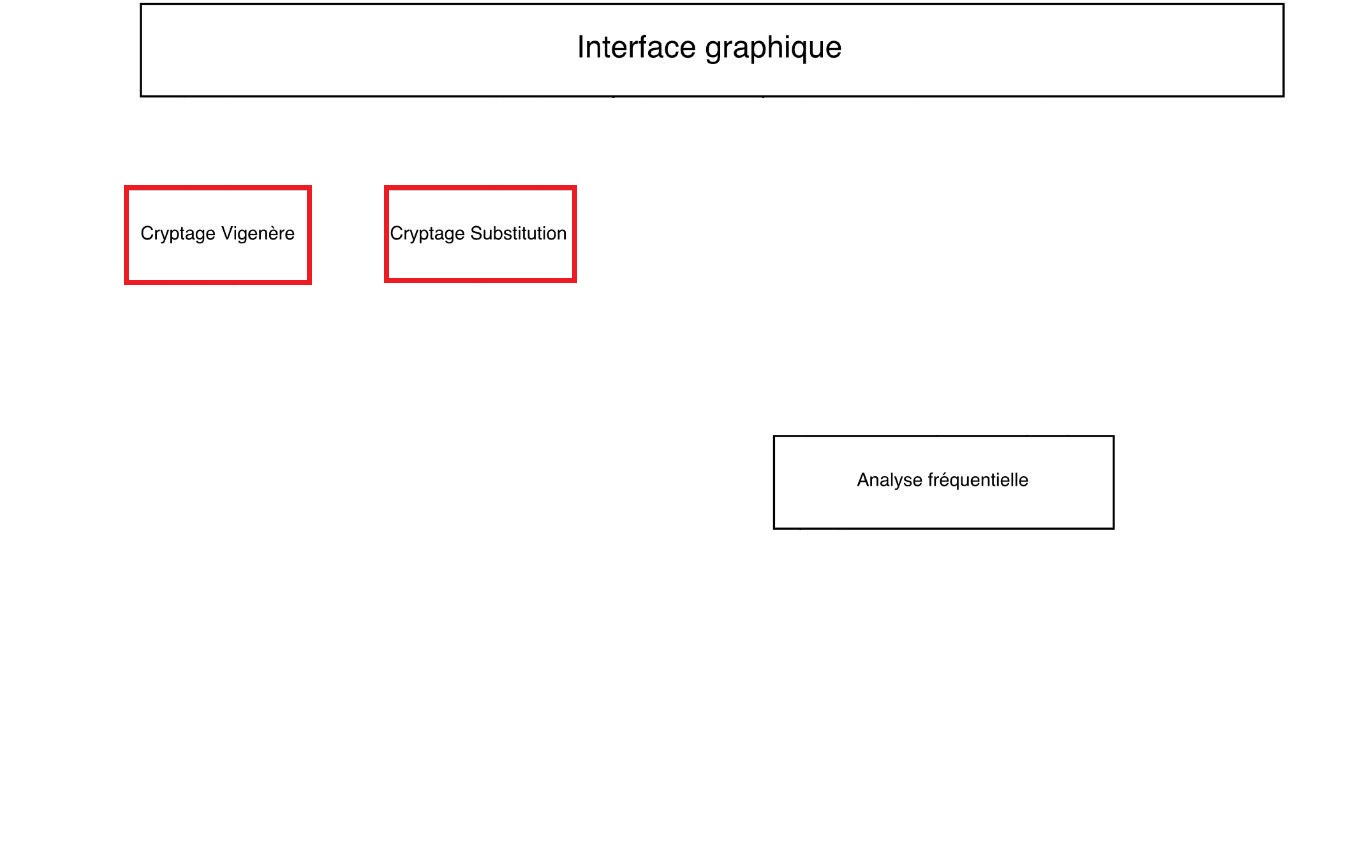
\includegraphics[scale = 0.28]{Org3.jpg}\\
Module permettant le cryptage d'un texte en clair et la génération de clefs de cryptage.
\end{frame}
\begin{frame}
  \frametitle{Organigramme}
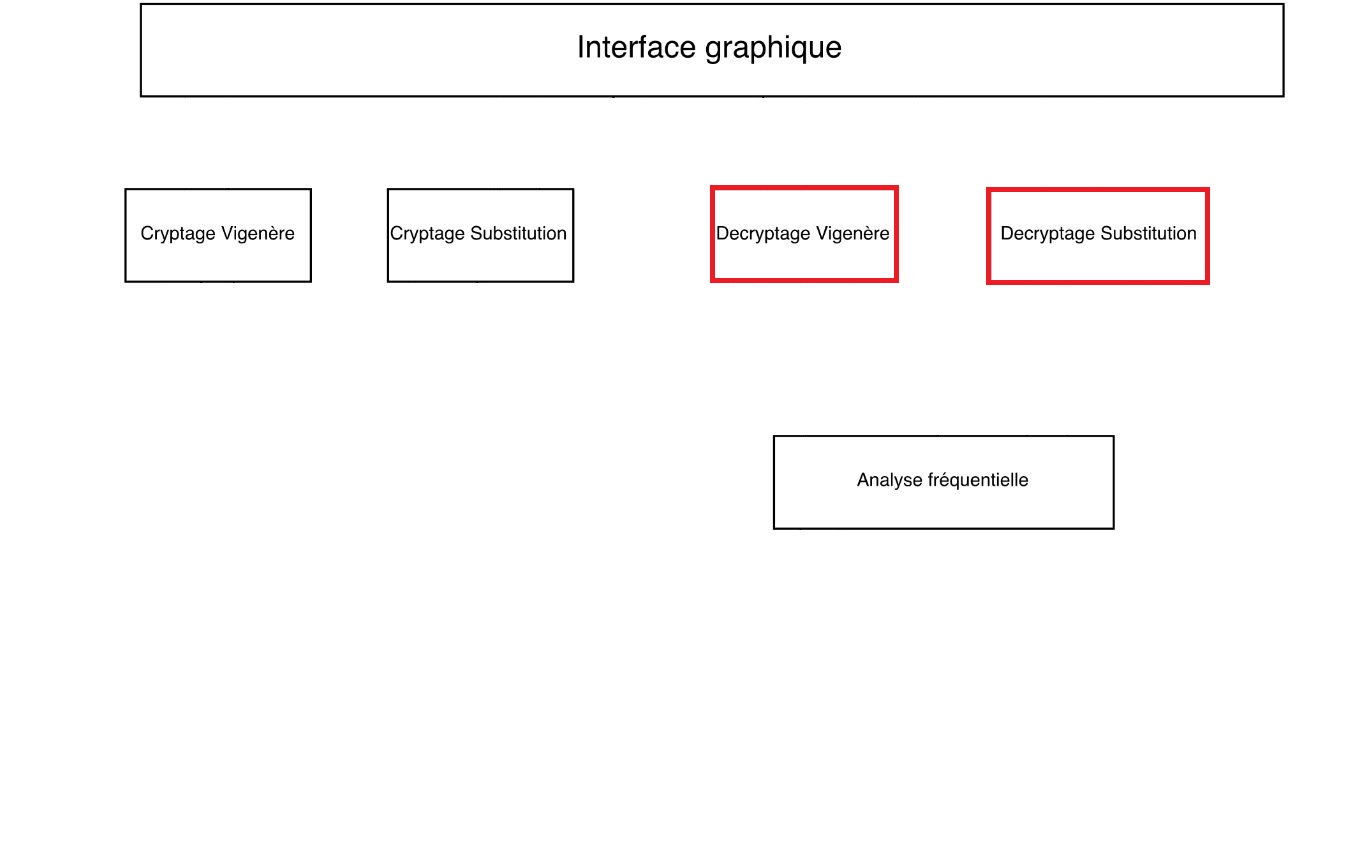
\includegraphics[scale = 0.28]{Org4.jpg}\\
Module qui permet le décryptage d'un texte crypté et la récuperation de clefs de cryptages.
\end{frame}
\begin{frame}
  \frametitle{Introduction}
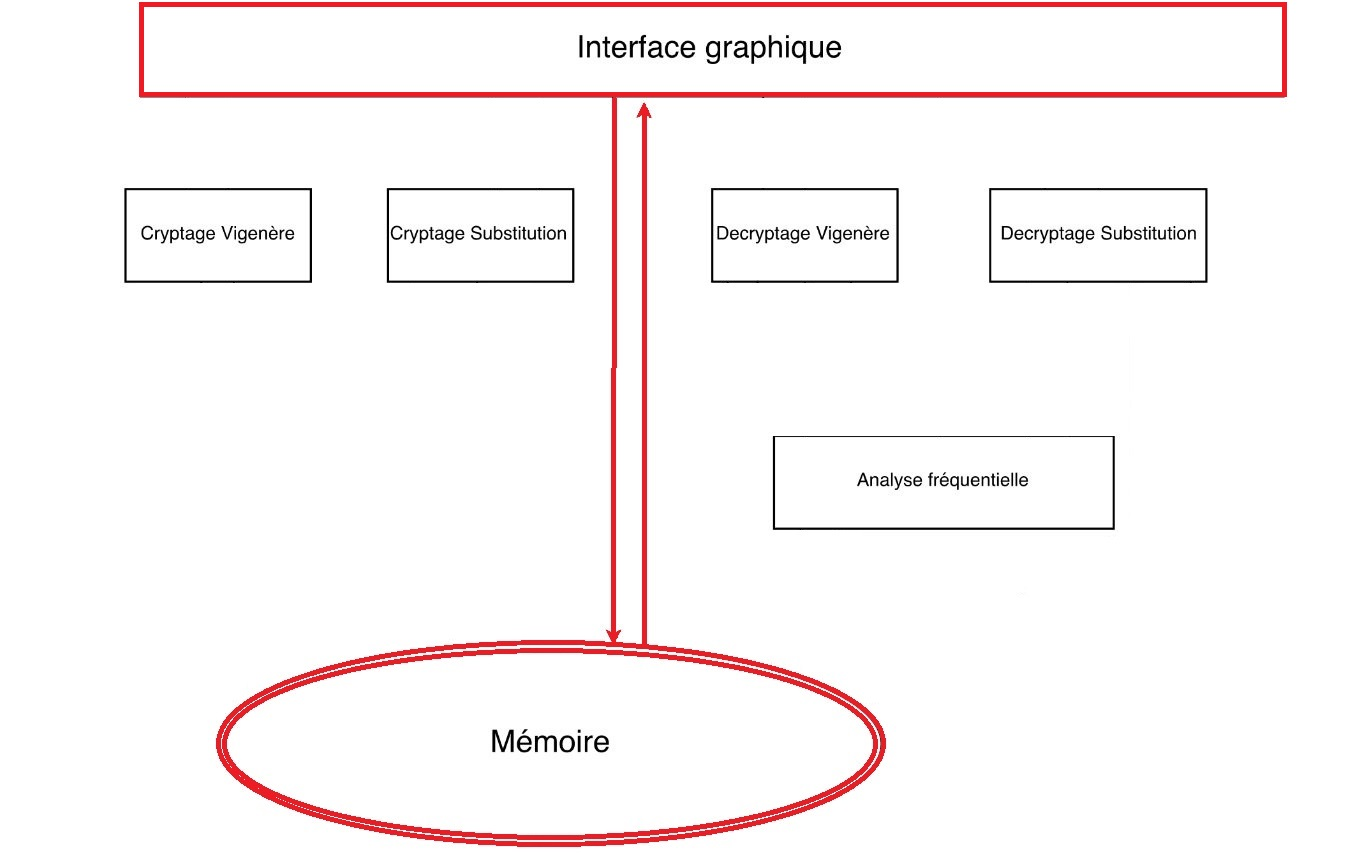
\includegraphics[scale = 0.28]{Org5.jpg}\\
L'interface graphique envoie un nom de fichier et reçoit le texte correspondant.
\end{frame}
\begin{frame}
  \frametitle{Organigramme}
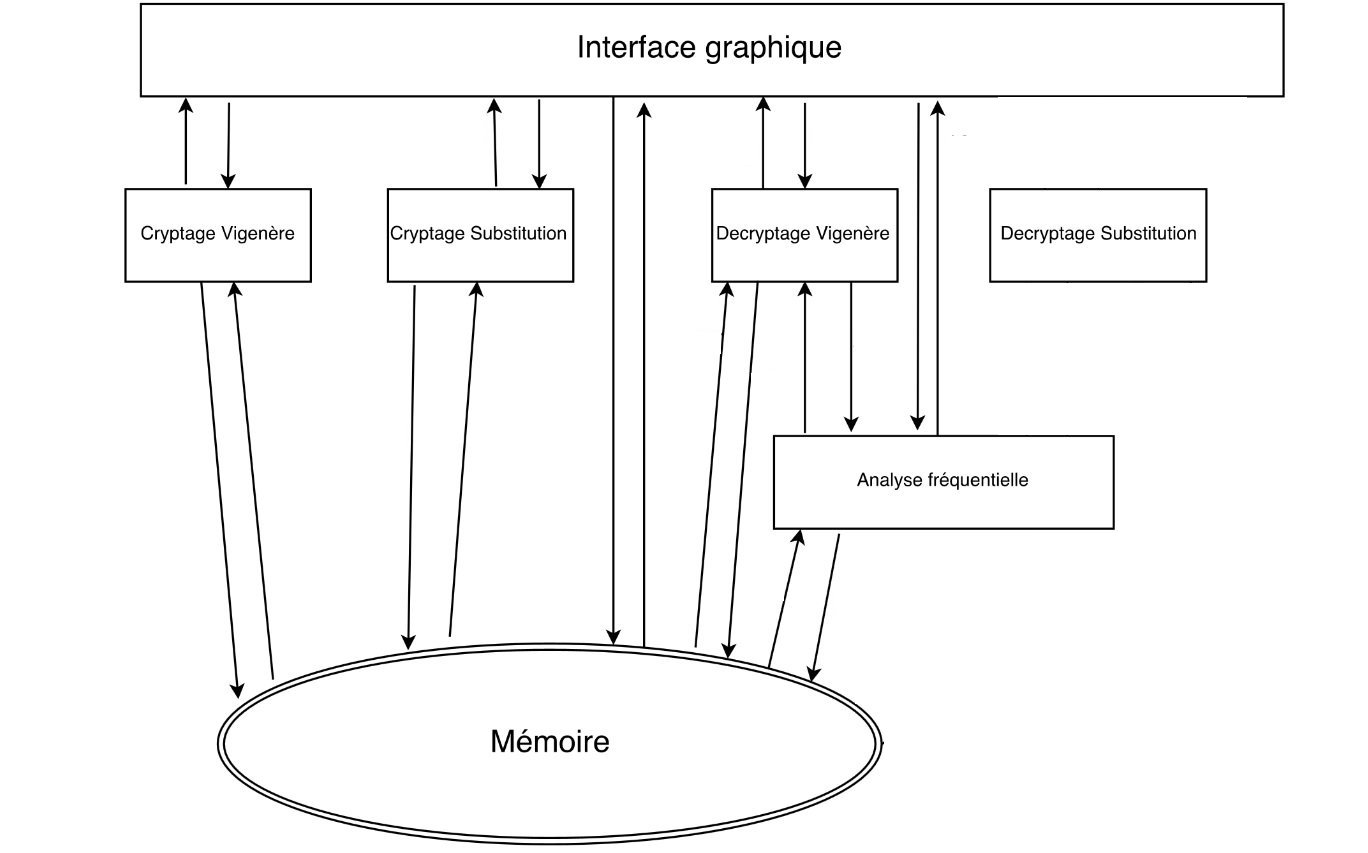
\includegraphics[scale = 0.28]{Org6.jpg}\\
L'interface graphique envoie une chaine de caractères et reçoit une structure contenant l'analyse fréquentielle.
\end{frame}
\begin{frame}
  \frametitle{Organigramme}
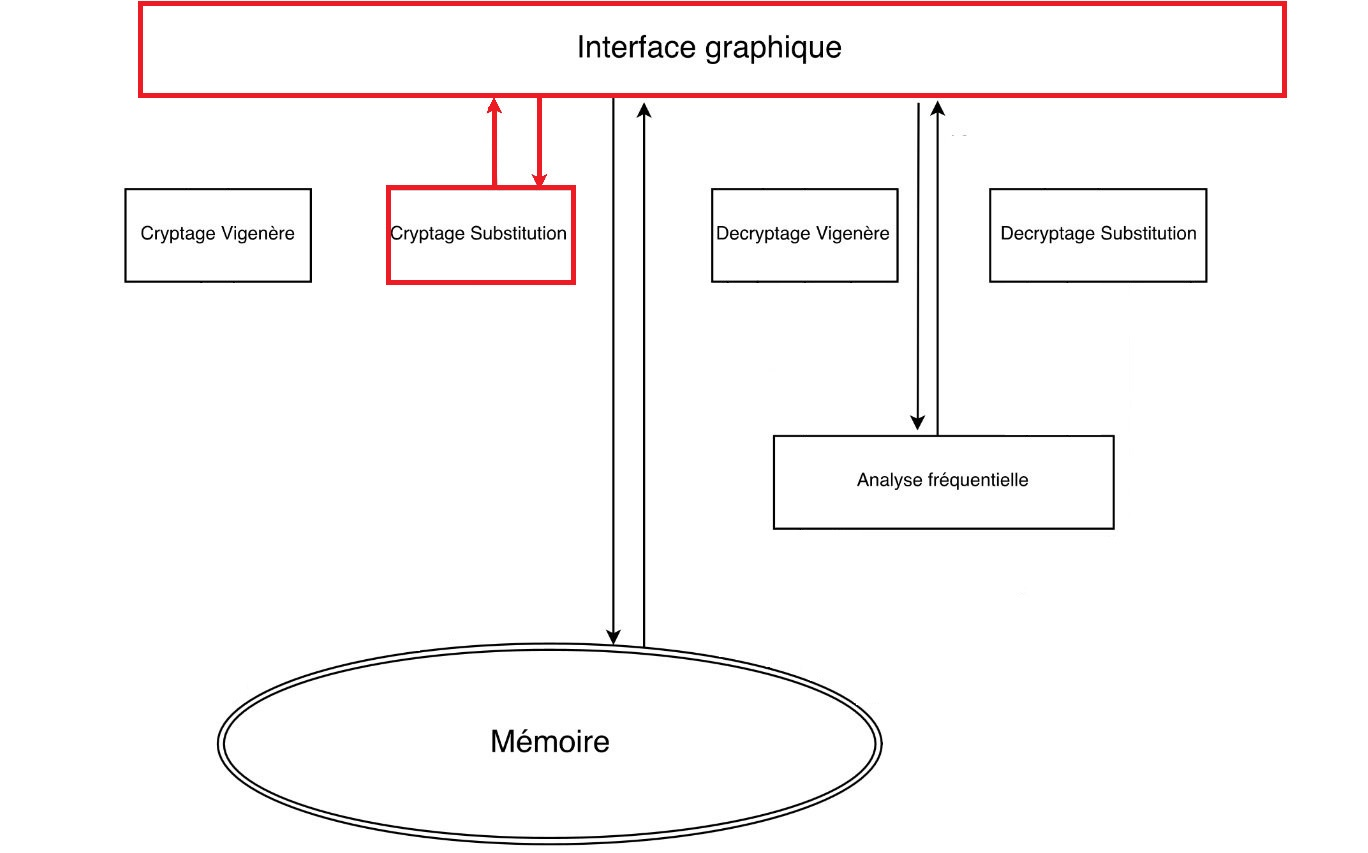
\includegraphics[scale = 0.28]{Org7.jpg}\\
L'interface graphique envoie trois chaines de caractères. Une contient 
le texte crypté et deux sont vides et seront remplies par le module de 
cryptage par substitution.
\end{frame}
\begin{frame}
  \frametitle{Organigramme}
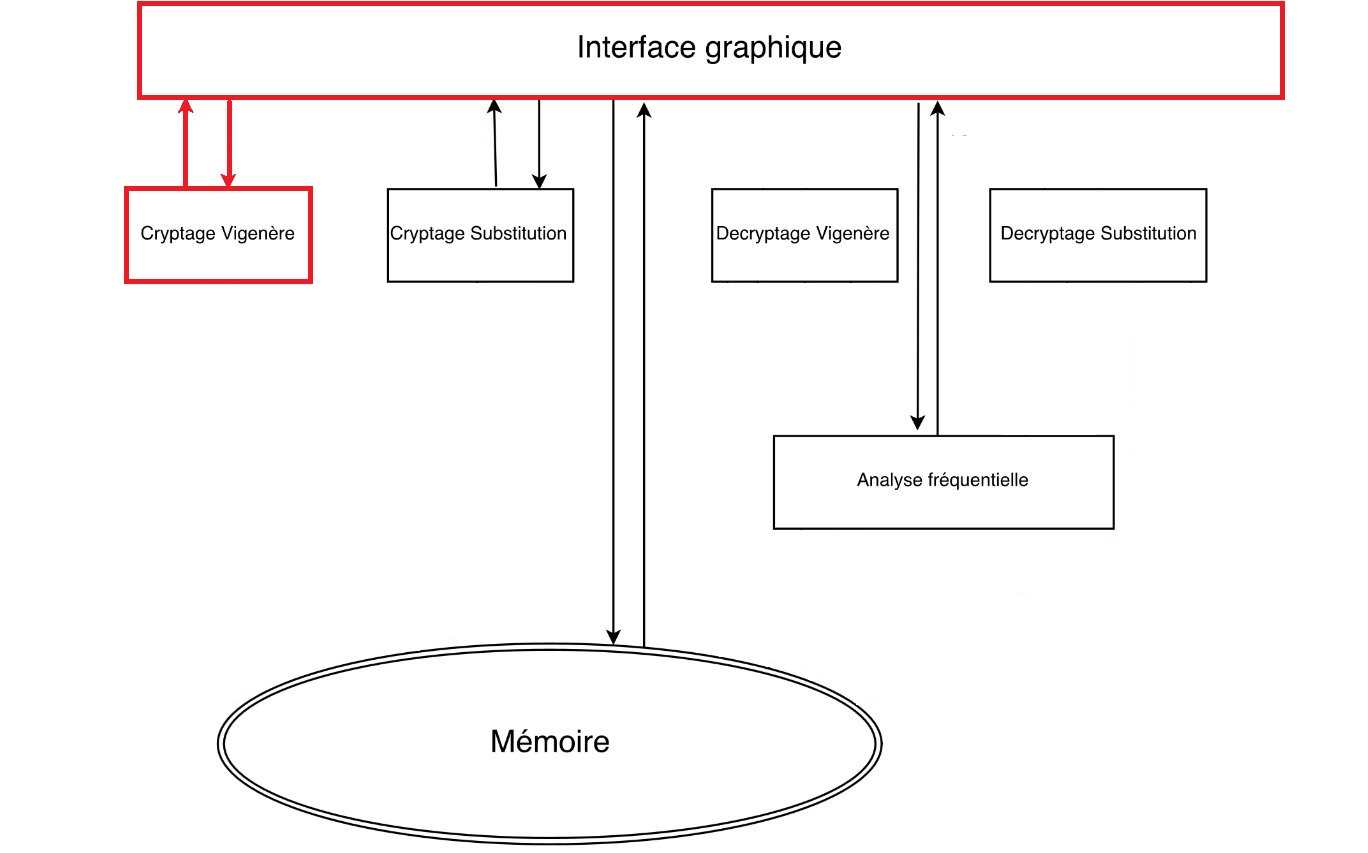
\includegraphics[scale = 0.28]{Org8.jpg}\\
Pour le cryptage par la méthode de vigenère l'interface graphique 
envoie trois chaines de caractères dont une contenant le texte 
en clair, une contenant la clef de cryptage et une vide qui sera remplie par 
le module.
\end{frame}
\begin{frame}
  \frametitle{Organigramme}
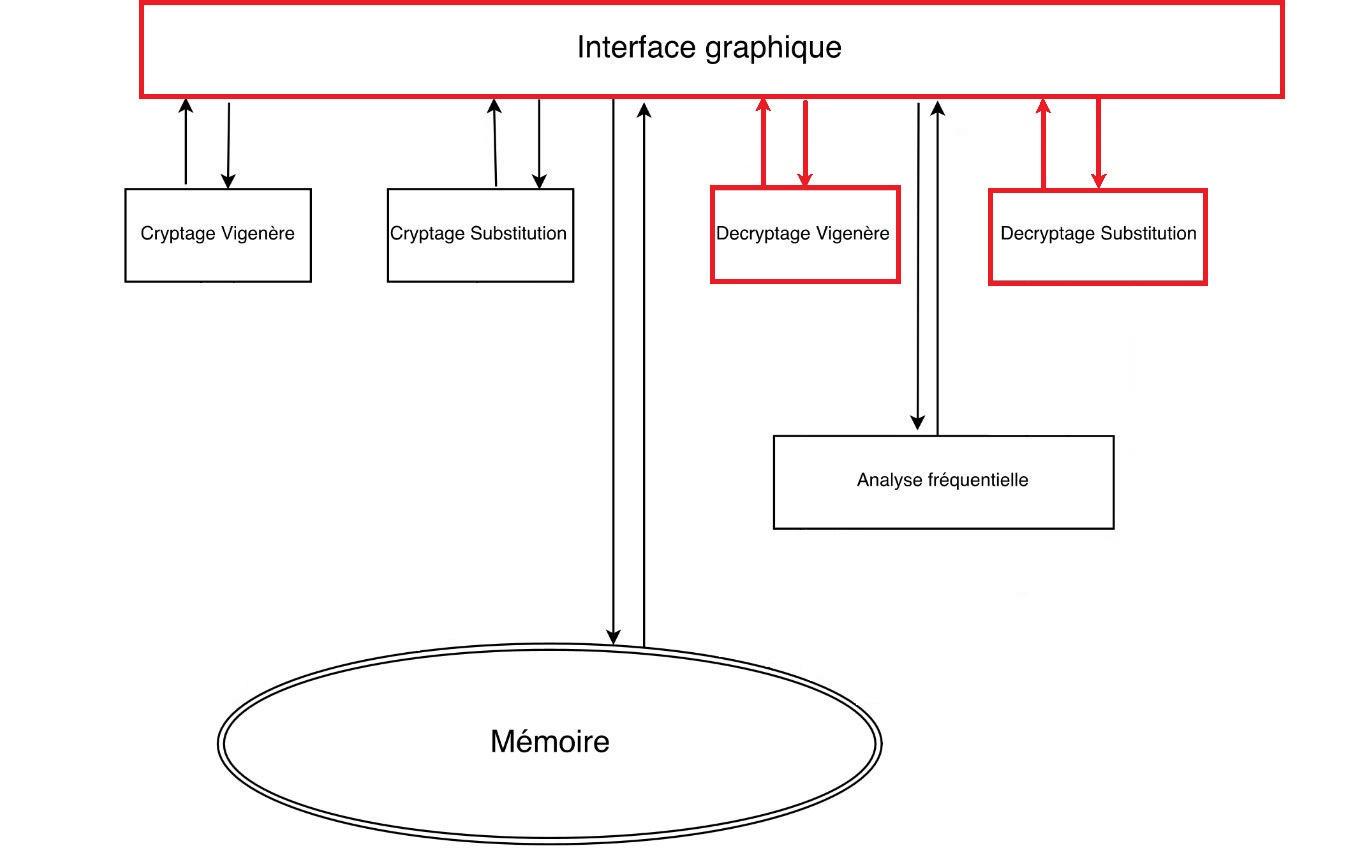
\includegraphics[scale = 0.28]{Org9.jpg}\\
Pour les deux decryptages, l'interface graphique envoie trois chaines de caractères.
 Une correspondant 
au texte crypté et deux vides qui seront remplies par les deux modules.
\end{frame}
\begin{frame}
  \frametitle{Organigramme}
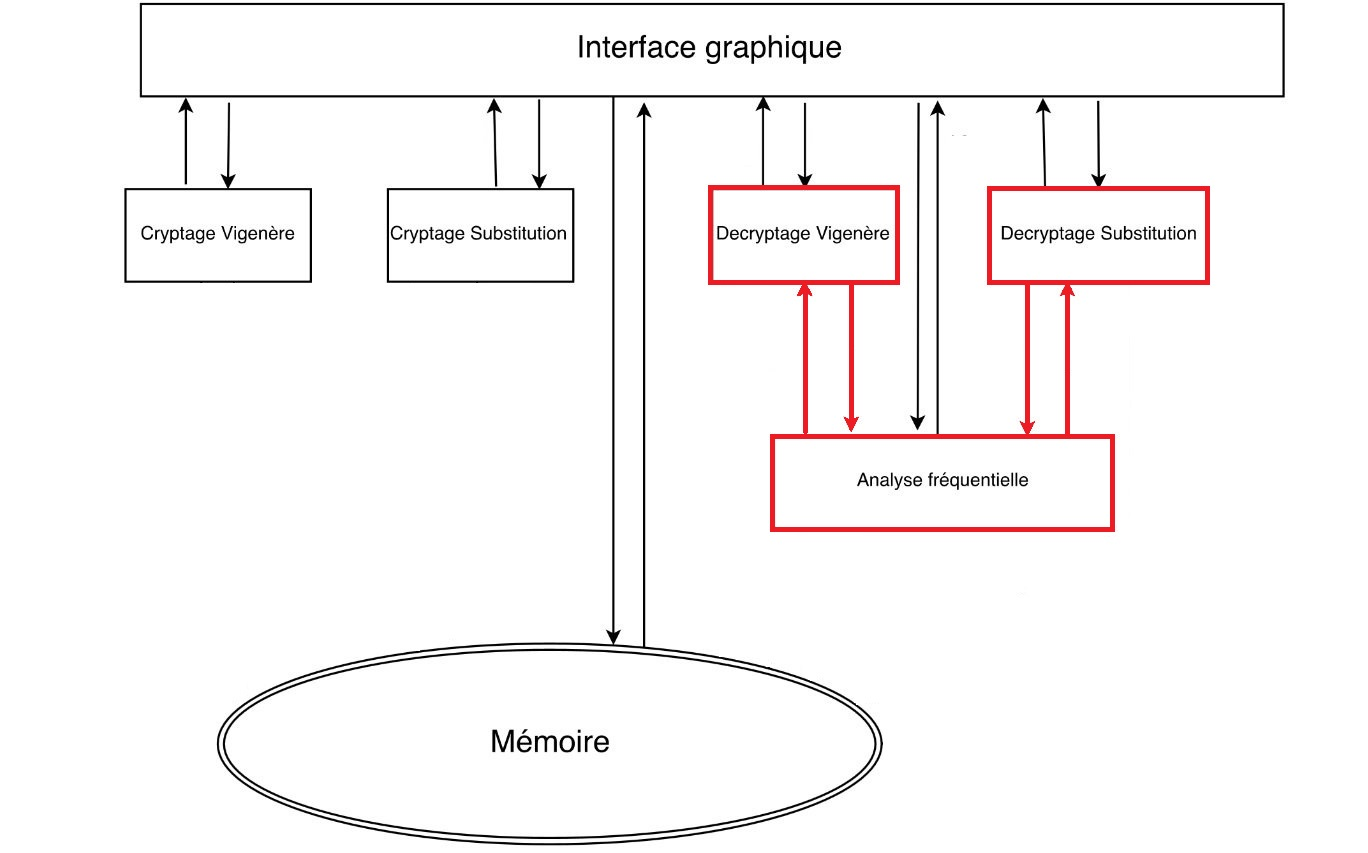
\includegraphics[scale = 0.28]{Org10.jpg}\\
L'analyse fréquentielle reçoit une chaine de caractères contenant le texte 
à analyser et renvoie une structure contenant l'analyse fréquentielle.
\end{frame}
%tibo
\begin{frame}
  \frametitle{Langage et bibliothèque graphique choisie}  
  \begin{block}{Les critères de la séléction du langage}
    \begin{itemize}
    \pause
  \item Besoin programmeur: \\
  -Traitement de données, langage performant et complet, installer l'application sur différents environnements. \\
  \pause
  \item Réponse: Le langage C \\
  -Programmation fonctionnelle(idéale pour traitement de données). \\
  -Langage performant et complet (source: IEEE)\\
  -Recompilation permet execution sur différents environnements.  \\
  \vspace*{1mm}
  \pause
   *De plus, langage C maitrisé par toute l'équipe. \\
    \end{itemize}
  \end{block}
 
  \pause
 
    \begin{block}{Les critères de séléction de la bibliothèque graphique}
    \begin{itemize}
    \pause
  \item Besoin de l'application: \\
                -Création de boutons, Zones de texte, Traitement de fichiers. \\
    \pause
  \item Réponse => GTK+ (The GIMP Toolkit) : ensemble de bibliothèques logicielles qui permettent la création d'une interface graphique.
        
  \item De plus, bibliothèque complète et non spécifique a un OS.
    \end{itemize}
  \end{block}
\end{frame}


\begin{frame}[<+->]
  \frametitle{Tests unitaires}
  \begin{block}{Utilisation de la librairie de Tests CUnit}
    \begin{itemize}
    \pause
  \item CUnit possède les fonctions nécessaires pour gèrer une suite de tests.
  \item Permet une maintenance et facilite l'amélioration de l'application
  \item Les tests lancent les fonctions de facon séparé avec un ASSERT qui vérifie par exemple si une variable contient le résultat attendu.\\
    \end{itemize}
  \end{block}
    \begin{block}{Exemple du lancement d'une suite test}
    \begin{center}
       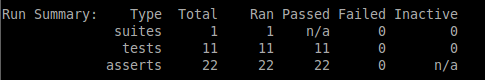
\includegraphics[scale = 0.6]{Capture.png}
    \end{center}
  \end{block}

\end{frame}
%younes
\begin{frame}[<+->]
  \frametitle{Partie technique}
	\begin{block}{Interface graphique}
	\begin{itemize}
		\item passage d'arguments\\ 
		\item switch\\ 
		\item erreur de mémoire suite à l'enregistrement
	\end{itemize}
	\end{block}
	\begin{block}{Analyse fréquentielle(Tri)}
	\begin{itemize}
		\item strcpy 
	\end{itemize}
	\end{block}
	\begin{block}{Decryptage Vigenere}
	\begin{itemize}
		\item kasiski\\ 
	\end{itemize}
	\end{block}
	\begin{block}{Decryptage Substitution}
	\begin{itemize}
		\item estimations\\ 
	\end{itemize}
	\end{block}
\end{frame}
%zak
\begin{frame}
 \frametitle{Organisation interne et repartition des taches}
\begin{block}{Tableau de repartition des taches}
\begin{center}
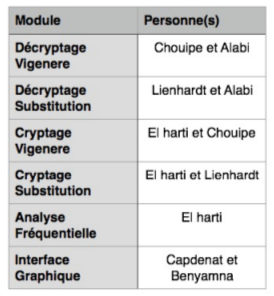
\includegraphics[scale =0.47]{taches.png} \\ 
\end{center}
\begin{itemize}
\item Organisation\\ 
\item Répartition des tâches respectée\\  
\item Avancement du projet\\ 
\end{itemize}
\end{block}
\end{frame}



\begin{frame}
\frametitle{Planing de développement}
\begin{block}{Points importants}
\begin{itemize}
\item L'interface graphique\\ 
\item Codage et tests de chaque module séparement\\ 
\item Assemblage de l'application\\ 
\item Priorité\\ 
\end{itemize}
\end{block}
\end{frame}




\begin{frame}
\frametitle{Nombre de lignes de code des modules}
\begin{block}{Tableau comparatif}
\begin{center}
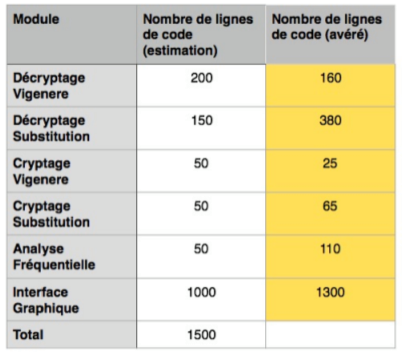
\includegraphics[scale =0.3]{tabl.png} \\ 
\end{center}
\end{block}
\end{frame}


\begin{frame}
\frametitle{Nombre de lignes de code des modules}
\begin{block}{Cryptage substitution}
\begin{center}
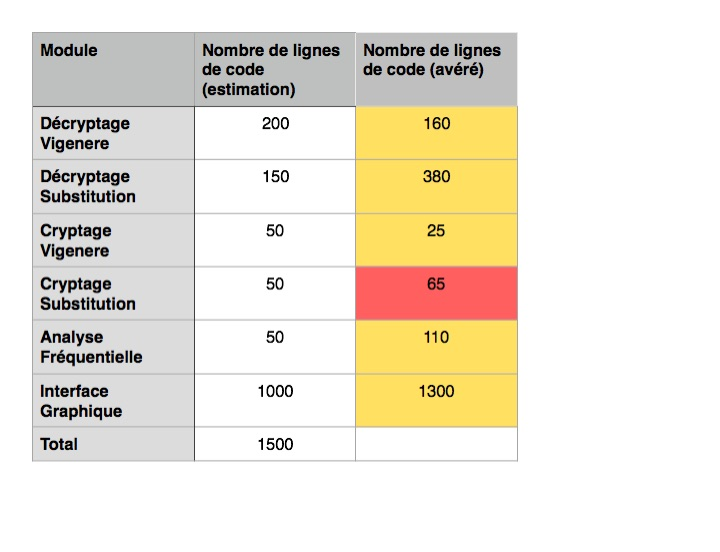
\includegraphics[scale =0.3]{preview.jpg} \\ 
\end{center}
\end{block}
\end{frame}

\begin{frame}
\frametitle{Nombre de lignes de code des modules}
\begin{block}{Analyse frequentielle}
\begin{center}
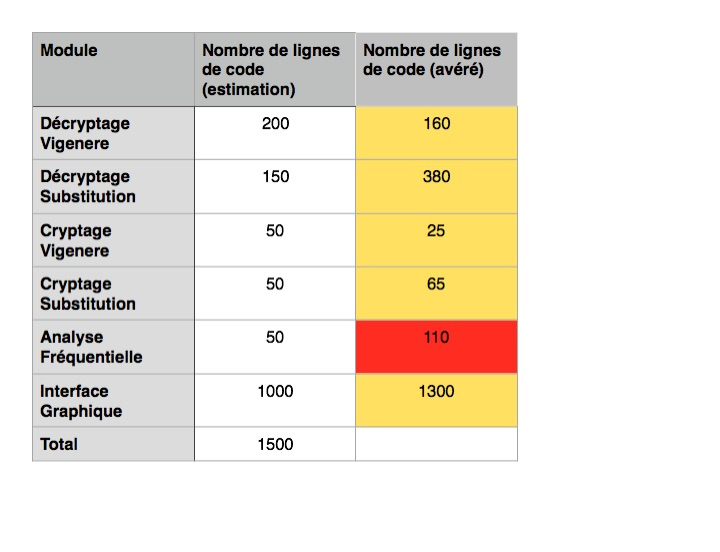
\includegraphics[scale =0.3]{preview2.jpg} \\ 
\end{center}
\end{block}
\end{frame}

\begin{frame}
\frametitle{Nombre de lignes de code des modules}
\begin{block}{Decryptage substitution}
\begin{center}
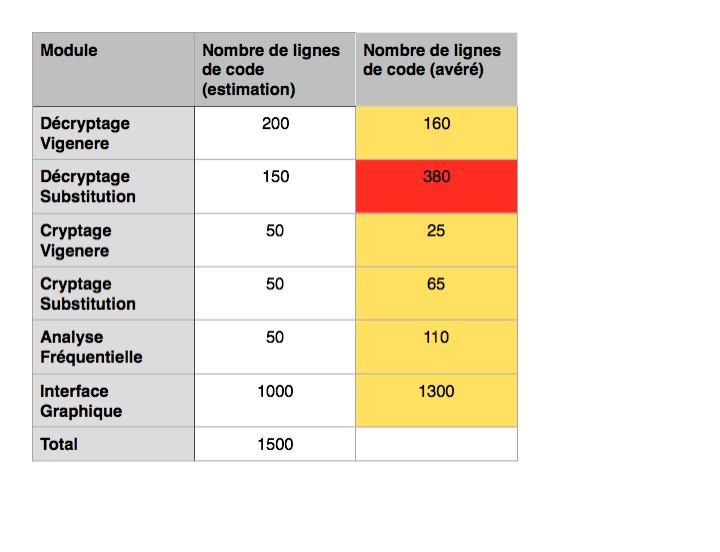
\includegraphics[scale =0.3]{preview3.jpg} \\ 
\end{center}
\end{block}
\end{frame}

\begin{frame}
\frametitle{Nombre de lignes de code des modules}
\begin{block}{Interface graphique}
\begin{center}
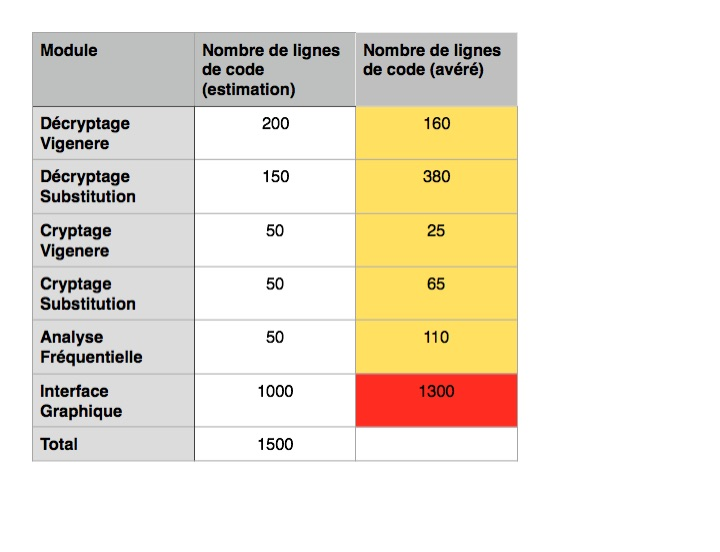
\includegraphics[scale =0.3]{preview4.jpg} \\ 
\end{center}
\end{block}
\end{frame}

%abio
\begin{frame}
  \frametitle{Conclusion}
	\begin{block}{Modifications et Ameliorations}
	\begin{itemize} \pause
		\item Ajouter un dictionnaire\\
		\item Modifier Cahier des Specifications\\ \pause
		\item Plus de langues\\ 
		\item Plus de choix de chiffrement
	\end{itemize}
	\end{block}
\end{frame}
\begin{frame}
  \frametitle{Conclusion}
\begin{center}

\includegraphics[scale =0.5]{logo.png}
\end{center}
\end{frame}


\end{document}
